\documentclass[a4paper,8pt,hyperref, aps, prl]{article}

\title{\bfseries \Large 
%Surface second harmonic generated by submilliwatt pump
%Surface second-order nonlinear effects with ultralow power
%Ultralow-pumped surface second-harmonic generation in centrosymmetric medium
Supplementary Information to surface second-harmonic generation enhanced by an ultrahigh-$Q$ microresonator
%of nonpolar media
}
\author{\normalsize  Xueyue Zhang$^{1,2}$, Qi-Tao Cao$^{1}$, Yu-xi Liu$^{2,3}$, Qihuang Gong$^{1,4}$, Yun-Feng Xiao$^{1,4,*}$ \\
  \\
\normalsize $^1$ State Key Laboratory for Mesoscopic Physics and School of Physics, Peking University \\
\normalsize Collaborative Innovation Center of Quantum Matter, Beijing 100871, People's Republic of China \\
\normalsize $^2$ Department of microelectronics and nanoelectronics, Tsinghua University, Beijing 100084, People’s Republic of China \\
\normalsize $^3$ Institute of Microelectronics, Tsinghua University, Beijing 100084, People’s Republic of China \\
\normalsize $^4$ Collaborative Innovation Center of Extreme Optics, Taiyuan 030006, Shanxi, People’s Republic of China \\
\normalsize $^*$ E-mail: yfxiao@pku.edu.cn
}
\date{\normalsize \today}

\usepackage[left=16mm,right=16mm, bottom = 16mm, top=20mm]{geometry}
\usepackage{upgreek}
\usepackage{hyperref}
\usepackage{booktabs}
\usepackage{tabularx}
\usepackage{xtab}
\usepackage{graphicx}
\usepackage{listings}
\usepackage{url}
\usepackage{amsmath}
%\usepackage{nature}



\lstset{
	flexiblecolumns,
	basicstyle = \sffamily,
	keywordstyle = \bfseries,
	commentstyle = \rmfamily\itshape,
	stringstyle = \ttfamily
}

\hypersetup{colorlinks=false}



%\pagestyle{myheadings}
%\markright{Name: Xueyue Zhang, GTID: 903181650}

\bibliographystyle{naturemag}

\begin{document}

\maketitle

\section{Theoretical model}

\textbf{Nonlinear coupling between the pump and the SH modes. }

The nonlinear coupling is the result of the excitation from the nonlinear polarization $\mathbf{P}$, which contains the surface and the bulk response $\mathbf{P} = \mathbf{P}^{\mathrm{surf}}_0+\mathbf{P}^{\mathrm{bulk}} = \mathbf{P}^{\mathrm{surf}}_0+\mathbf{P}^{\mathrm{bulk}}_\gamma+\mathbf{P}^{\mathrm{bulk}}_\delta$. 
The nonlinear coefficients $\gamma$ and $\delta$ represents the bulk multipole response with different forms $\mathbf{P}^{\mathrm{bulk}}_\gamma =  \gamma\nabla(\mathbf{E}\cdot\mathbf{E})$ and $\mathbf{P}^{\mathrm{bulk}}_\delta = \delta(\mathbf{E}\cdot\nabla)\mathbf{E}$ \cite{bloembergen1968optical}, where $\mathbf{E}$ is the electric field. 
The former one, as a longitudinal wave, only contributes at the surface, which can be written as an effective surface nonlinear susceptibility tensor with two non-zero components $\upchi_{\gamma \perp \perp \perp}$ and $\upchi_{\gamma \perp \parallel \parallel}$ \cite{heinz1991second}. 
$\mathbf{P}^{\mathrm{surf}}_0+\mathbf{P}^{\mathrm{bulk}}_\gamma$ can be written into an effective surface polarization $\mathbf{P}^{\mathrm{surf}}$ with the corresponding susceptibility $\upchi^{(2)}_s = \upchi^{(2)}_{s0}+\upchi^{(2)}_{s,\gamma}$
\label{eq:Pdef}
\begin{equation}
\mathbf{P}^{\mathrm{surf}} = \epsilon_0\upchi^{(2)}_s:\mathbf{E}_1\mathbf{E}_1,
\end{equation}
where $\mathbf{E}_1$ is the pump electric field and $\epsilon_0$ the vacuum permittivity. The Helmholtz equation for the SH electric field $\mathbf{E}_2$ can be written as 
\begin{equation}
(\nabla^2 -\frac{n_2^2}{c^2}\frac{\partial^2}{\partial t^2})\mathbf{E}_{2} = \frac{1}{\epsilon_0c^2}\frac{\partial^2(\mathbf{P}^{\mathrm{surf}}+\mathbf{P}^{\mathrm{bulk}}_\delta)}{\partial t^2}
\label{eq:Helm}
\end{equation}
where $n_2$ is the refractive index and $c$ is the speed of light in the vacuum. 

The electric field $\mathbf{E}_j$ ($j = 1,2$) in a microresonator exhibits the form of $\mathbf{E}_j (\mathbf{x}, t) = \tilde{\alpha}_j (t) \mathbf{E}_{0j} (\mathbf{x}) e^{-i\omega_j t}$, where $\tilde{\alpha}_j (t)$ is the slowly varying field amplitude and $|\tilde{\alpha}_j (t)|^2$ corresponds to the intracavity energy, $\mathbf{E}_{0j} (\mathbf{x})$ represents the normalized field distribution, $\omega_j$ is the frequency of the field. 
Note that $\mathbf{E}_{0j}$ is a mode of the resonator, which gives
\begin{equation}
(\nabla^2 -\frac{n_2^2}{c^2}\frac{\partial^2}{\partial t^2})(\mathbf{E}_{02}e^{-i\omega_2 t}) = 0
\label{eq:eigen}
\end{equation}
Equations (\ref{eq:Pdef})-(\ref{eq:eigen}) yields
\begin{gather}
\frac{d \tilde{\alpha}_2}{dt} =  i(g_{s}+g_{b})\tilde{\alpha}_1^2e^{-i(2\omega_1-\omega_2)t}, \\
g_{s}  = 2\frac{\omega_1^2}{\omega_2n_2^2}\frac{\int_{\mathrm{surface} } \mathbf{E}_{02}^* \cdot \upchi^{(2)}_{s}:\mathbf{E}_{01}\mathbf{E}_{01} \mathrm{d}	\mathbf{S}}{\int |\mathbf{E}_{02}|^2 \mathrm{d}	\mathbf{V}}, \label{eq:gs} \\
g_b =  2\frac{\omega_1^2}{\omega_2n_2^2}\frac{\delta \int \mathbf{E}_{02}^* \cdot (\mathbf{E}_{01}\cdot\nabla)\mathbf{E}_{01} \mathrm{d}	\mathbf{V}}{\int |\mathbf{E}_{02}|^2 \mathrm{d} \mathbf{V}}
\label{eq:gb}
\end{gather}
The slowly varying approximation ($\frac{d^2\tilde{\alpha}_j}{dt^2} \ll \omega_j\frac{d\tilde{\alpha}_j}{dt}$ and $\frac{d\tilde{\alpha}_j}{dt} \ll \omega_j$) is assumed in the derivation. The volume integration is replaced by the surface integration in equation (\ref{eq:gs}) since the surface polarization is zero except for the surface. Equations (\ref{eq:gs}) and (\ref{eq:gb}) are exactly the same with equations (2) and (3) in the main text.

Considering the lossless coupling ($d|\tilde{\alpha}_1|^2/dt+d|\tilde{\alpha}_2|^2/dt=0$), the nonlinear coupling induced changing rate for $\tilde{\alpha}_1|$ can be written as 
\begin{equation}
\frac{d \tilde{\alpha}_1}{dt} =  -i(g_{s}+g_{b})^*\tilde{\alpha}_1^*\tilde{\alpha}_2e^{-i(\omega_2-2\omega_1)t}
\end{equation}

\textbf{Coupled mode equations}

Incorporating the loss and the input power gives the full coupled mode equations
\begin{gather}
\frac{d{\tilde{\alpha}_1}}{dt} = -\frac{\kappa_{10}+\kappa_{1e}}{2}\tilde{\alpha}_1+\sqrt{\kappa_{1e}}se^{-i(\omega_p-\omega_1)t}-ig^*\tilde{\alpha}_1^*\tilde{\alpha}_2e^{-i(\omega_2-2\omega_1)t} \label{eq:cpmode1}\\
\frac{d\tilde{\alpha}_2}{dt} = -\frac{\kappa_{20}+\kappa_{2e}}{2}\tilde{\alpha}_2+ig\tilde{\alpha}_1^2e^{-i(2\omega_1-\omega_2)t}
\label{eq:cpmode2}
\end{gather}
where $g=g_s+g_b$ is the total nonlinear coupling strength, $\omega_p$ and $s$ are the frequency and the amplitude of the input electric field in the pump fiber with $|s|^2$ the input power, $\kappa_{j0}$ and $\kappa_{je}$ represent the intrinsic and external coupling rate respectively.

In the rotating frame of the pump, using ${\alpha}_1 = \tilde{\alpha}_1e^{i(\omega_p-\omega_1)t}$ and ${\alpha}_2 = \tilde{\alpha}_2e^{i(2\omega_p-\omega_2)t}$, the coupled mode equations can be rewritten as
\begin{gather}
\label{eq:cpmoder1}
\frac{d{\alpha}_1}{dt} = [i(\omega_p-\omega_1)-\frac{\kappa_{10}+\kappa_{1e}}{2}]{\alpha}_1+\sqrt{\kappa_{1e}}s-ig^*{\alpha}_1^*{\alpha}_2 \\
\frac{d{\alpha}_2}{dt} = [i(2\omega_p-\omega_2)-\frac{\kappa_{20}+\kappa_{2e}}{2}]{\alpha}_2+ig{\alpha}_1^2
\label{eq:cpmoder2}
\end{gather}
which are the same with equations (4) and (5) in the Methods.

Assume that the pump is unperturbed by the generation of SH, which is true when the SH is weak. The last term in equation (\ref{eq:cpmoder1})  can be ignored in further analysis. In the steady state, the above coupled mode equations results in the expression of generated SH power
\begin{equation}
P_2 = \frac{4|g|^2\kappa_{2e}Q_2^2/\omega_2^2}{4Q_2^2(2\omega_p/\omega_2-1)^2+1}\frac{16\kappa_{1e}^2Q_1^4/\omega_1^4}{[4Q_1^2(\omega_p/\omega_1-1)^2+1]^2}P_1^2
\end{equation}
where $Q_j = \omega_j/(\kappa_{j0}+\kappa_{je})$ is the loaded quality factor. The above equation is the same as equation (1) in the main text.

\textbf{Quantum selection rule and the vanishing of $\mathbf{P}^{\mathrm{bulk}}_\delta$} 

In a microsphere, the quantum selection rule requires the coupling pair of modes to have certain angular and azimuthal numbers ($l_j$ and $m_j$ respectively). 
\begin{equation}
0 \le l_2 \le 2l_1, m_2 = 2m_1
\end{equation}
According to the above equation, the fundamental pump modes with $l_1 = m_1$ can only couple with the fundamental SH modes since $l_2 \le 2l_1 = 2m_1 = m_2$ and $l_2 \ge m_2$.

For TE polarized pump, the divergence in equation (\ref{eq:gb}) is along the polar direction, and $(\mathbf{E}_{01}\cdot\nabla)\mathbf{E}_{01}$ results in an odd function in the polar direction no matter which parity $\mathbf{E}_{01}$ exhibits in this direction.


\textbf{Thermal effects and optical Kerr effect}

Thermal effects denote the thermal expansion and refractive index change, both of which can be included in an effective refractive index change coefficient $({\partial n}/{\partial T})_{\mathrm{eff}}$ \cite{carmon2004dynamical} and written into a nonlinear polarization $\mathbf{P}^{\mathrm{thm}} = \epsilon_0[2n_j(\partial n/{\partial T})_\mathrm{eff}\Delta T]\mathbf{E}_j$. Here $\Delta T (\mathbf{x},t)$ is the change of temperature distribution. The Kerr effect can also be treated with a nonlinear polarization $\mathbf{P}^{\mathrm{Kerr}}$. Introduce the nonlinear polarizations into  the Helmholtz equation for the pump and the SH, and we can obtain the shifted resonance frequency $\omega_1 =\omega_{10} -B_{11}|\alpha_1|^2$ and $\omega_2 =\omega_{20} -B_{12}|\alpha_1|^2$ with 
\begin{gather}
\label{eq:B11}
B_{11} = [\frac{3\upchi_{\mathrm{Kerr}}\omega_1}{n_1^2}+(\frac{\partial n}{\partial T})_{\mathrm{eff} }\frac{\epsilon_0}{\rho C \delta_{T}}\frac{\omega_1^2n_1}{Q_{1,\mathrm{abs}}}]\frac{\int|\mathbf{E}_{01}|^4d\mathbf{V}}{\int|\mathbf{E}_{01}|^2d\mathbf{V}}, \\
B_{12} = [\frac{6\upchi_{\mathrm{Kerr}}\omega_2}{n_2^2}+(\frac{\partial n}{\partial T})_{\mathrm{eff} }\frac{\epsilon_0}{\rho C \delta_{T}}\frac{\omega_1\omega_2n_1^2}{n_2Q_{1,\mathrm{abs}}}]\frac{\int|\mathbf{E}_{01}|^2|\mathbf{E}_{02}|^2d\mathbf{V}}{\int|\mathbf{E}_{02}|^2d\mathbf{V}}
\label{eq:B12}
\end{gather}
where $\upchi_{\mathrm{Kerr}}$ is the Kerr nonlinear susceptibility, $\rho$ denotes the density of cavity, $C$ is the specific heat capacity, $\delta_{T}$ represents the thermal relaxing rate \cite{fomin2005nonstationary}, and $Q_{1,\mathrm{abs}}$ is the cavity quality factor due to absorption loss, which is the source of optical power induced heating. The thermal and Kerr effects of the SH is ignored assuming the power of SH is much smaller than the pump.

Using the equations (\ref{eq:B11}) and (\ref{eq:B12}), the rates of frequency change can be compared for the SH mode and the SH signal. If the temperature and intracavity power is homogeneous, $B_{12} \approx 2B_{11}$ due to the scaling of $\omega_j$. With the pump light as the source of resonance shift, the temperature and intracavity power distribution overlaps perfectly with the pump mode but not as good with the SH mode. Therefore, $B_{12} < 2B_{11}$ as can be seen from the overlap integral in equations (\ref{eq:B11}) and (\ref{eq:B12}). As an example, the coefficients are calculated within a microsphere (diameter = $62$ $\upmu$m) using a pair of modes that are nearly phase matching and can generate second harmonic. The pump mode is a fundamental mode with radial ($q_1$), angular ($l_1$) and azimuthal ($m_1$) numbers equal to 1, 171 and 171 respectively. And for the SH mode, $q_2=2$ and $l_2 = m_2 = 342$. In this case, $2B_{11}/B_{12} = 1.052$. Furthermore,        it is obvious to see $\Delta \omega_2<2\Delta \omega_1<2\Delta \omega_p$, which is the condition for the SH signal to catch the SH mode in the phase-matching process.

\section{Power dependence induce by thermal and Kerr assisted phase-matching}

As is described in the main text, the thermal and Kerr assisted phase-matching method introduces a critical power in SHG. The process to obtain the power dependence curve (Fig. \ref{pic:FigS1}a) is illustrated in Fig. \ref{pic:FigS1}b. With different the pump wavelengths, the maximum SH power is recorded as shown by the blue dots. Note that both in the measurement and the theoretical calculation, the SH power at any detuning is recorded in a steady state. 
Further increase of the SH power is limited by the larger detuning between the pump and the thermally-shifted pump cavity mode. 
The inset in Fig. \ref{pic:FigS1}a shows the almost unchanged intracavity power and the pump wavelength with maximum SH power, which results in the almost unchanged SH power with increasing pump power above the critical power. 
To confirm that the increasing of intracavity power is negligible with increasing input power at a certain pump wavelength, we measure the resonance shift of a mode near 780 nm at i) increasing input power at a fixed pump wavelength, ii) increasing pump wavelength at a fixed pump power. The resonance shift in the first case is almost unresolvable with the oscilloscope, which represents an almost unchanged intracavity power in this case.

\begin{figure}[!ht]
\centering
%\captionsetup{singlelinecheck=no, justification = RaggedRight}
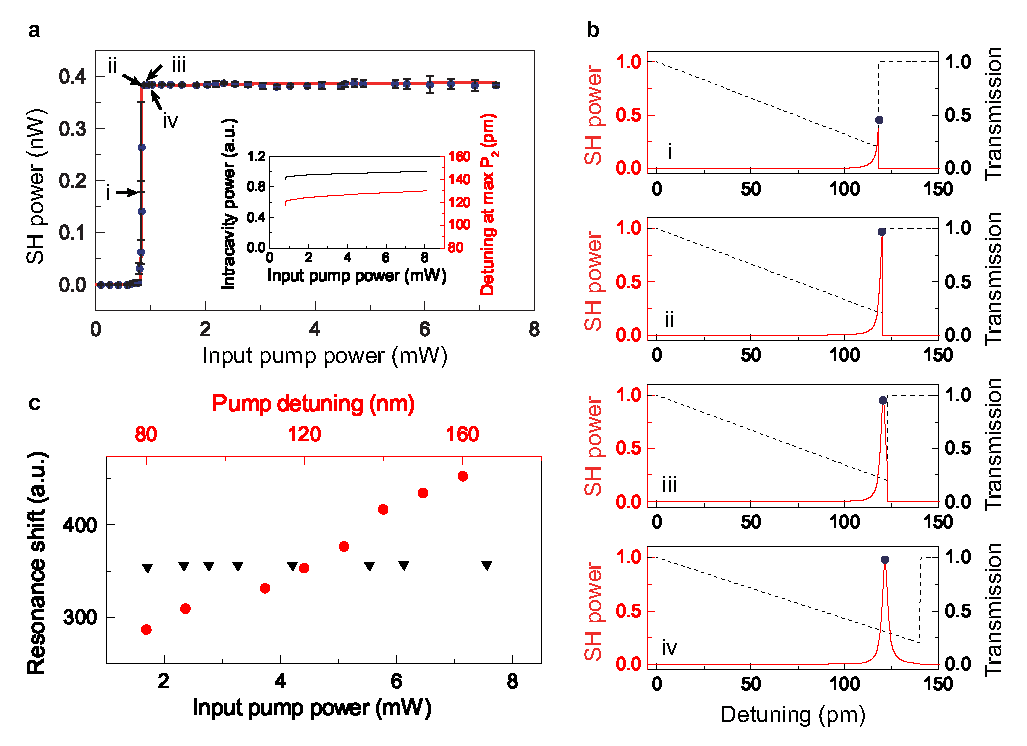
\includegraphics[width=16cm]{FigS1.eps}
\caption{\textbf{Dependence of SH power on the pump power. a, }Measured and theoretical SH power versus the input pump power (the same as Fig. 2\textbf{d} in the main text). Inset: Theoretically calculated intracavity power (black) and the pump-cold-cavity-mode detuning (red) with maximum SH power versus the input power. \textbf{b, }Theoretically calculated SH power (red solid curve) and the pump transmission (black dashed curve) versus the detuning at four fixed input power corresponding to i-iv in \textbf{a.} \textbf{c, } Measured resonance shift of a mode near 780 nm with changing input power at the detuning of 120 pm (black triangle) and with changing detuning at the pump power of 1.7 mW (red circle).}
\label{pic:FigS1}
\end{figure}

\section{An alternative way to identify the surface or bulk nonlinear response}

Besides the method of pumping a TE fundamental mode, the contribution from the surface or the bulk can also be clarified by measuring the polarization of the generated SH signal under the TE pump. Note that equation (\ref{eq:gb}) requires the pump and the SH to exhibit the same polarization while the tensor $\upchi^{(2)}_s$ in equation (\ref{eq:gb}) can be reduced to $\upchi_{\parallel \parallel \perp}$ in the TE pump case, which can only generate SH with TM polarization. 
Additionally, $\mathbf{P}^{\mathrm{bulk}}_\gamma$ is also absent in the  susceptibility $\upchi_{\parallel \parallel \perp}$. 
Therefore, with the determination of the SH polarization, we can obtain both surface-only and bulk-only SH signals.



\bibliography{ref}


\end{document}

